\documentclass{l4proj}
\usepackage{enumitem}
\usepackage{booktabs}   
%
% put any additional packages here
%

\begin{document}

%==============================================================================
%% METADATA
\title{A Self-Driving Robot Competition and Controller for Autonomous Robots}
\author{Lewis Trundle}
\date{March 24, 2023}

\maketitle

%==============================================================================
%% ABSTRACT
\begin{abstract}
    Every abstract follows a similar pattern. Motivate; set aims; describe work; explain results.
    \vskip 0.5em
    ``XYZ is bad. This project investigated ABC to determine if it was better. 
    ABC used XXX and YYY to implement ZZZ. This is particularly interesting as XXX and YYY have
    never been used together. It was found that  
    ABC was 20\% better than XYZ, though it caused rabies in half of subjects.''
\end{abstract}

%==============================================================================

% EDUCATION REUSE CONSENT FORM
\def\consentname {Lewis Trundle}
\def\consentdate {24 March 2023}
\educationalconsent


%==============================================================================
\tableofcontents

%==============================================================================
%% Notes on formatting
%==============================================================================
% The first page, abstract and table of contents are numbered using Roman numerals and are not
% included in the page count. 
%
% From now on pages are numbered
% using Arabic numerals. Therefore, immediately after the first call to \chapter we need the call
% \pagenumbering{arabic} and this should be called once only in the document. 
%
% Do not alter the bibliography style.
%
% The first Chapter should then be on page 1. You are allowed 40 pages for a 40 credit project and 30 pages for a 
% 20 credit report. This includes everything numbered in Arabic numerals (excluding front matter) up
% to but excluding the appendices and bibliography.
%
% You must not alter text size (it is currently 10pt) or alter margins or spacing.
%
%
%==================================================================================================================================
\chapter{Introduction}
% reset page numbering. Don't remove this!
\pagenumbering{arabic} 

\section{Motivation}
Since its conception decades ago, the field of autonomous robotics has been a popular area of study, with applications in areas such as healthcare, manufacturing, and transportation. However, in recent years, it has become increasingly popularised in the entertainment industry, with competitions such as the AWS DeepRacer League bringing in an influx of thousands of viewers and competitors every year. With new robotic competitions appearing every year, these competitions present a way for keen enthusiasts of autonomous robotics to showcase their skills in their area of interest by solving challenges, and collaborating with other enthusiasts to help improve their community.
\\\\
However, despite this growing popularity, there still lacks competitions which demonstrate both affordability and accessibility, as well as promoting collaboration. Many platforms require physical participation and can quite often be costly - requiring expensive robots or services. For example, the DeepRacer project, although not required, heavily suggests using Amazon's hardware, which can cost hundreds of dollars. Although to a company this may not seem like much, it can be a massive barrier in those with little access to these types of resources. Additionally, many competitions have no requirement that solutions must be made available to the public, meaning those with resources available to spend can keep winning solutions private. These factors all contribute towards the autocratization of autonomous robotics, where large, well-funded companies dominate these competitions, leaving no room for small-scale, independent enthusiasts.
\\\\
An additional crucial aspect of these competitions is their allowance to use a wide-variety of autonomous driving techniques. This versatility is essential in allowing participants to learn and share a wide variety of different skills which address the given challenges. However, many existing competitions restrict their participants to only using one specific approach, such as the DeepRacer where participants must use machine learning.
\\\\
These restrictions limit the opportunities for many to participate in the growing field of autonomous robotics. Their unaffordability dissuades individuals such as students from entering due to its costly nature, and their inaccessibility discourages those from different places around the world. Combined, these factors dampen the development of diverse ideas and hinders collaboration and discussion. With this in mind, the autonomous robotics community could benefit from a new competition - one which is inexpensive, available to anyone to enter, promotes collaboration, and allows a wide variety of diverse approaches.

\section{Project Aim}
Following from Motivation 1.1 the overall aim of this project is to create such a competition for a self-driving robot and prove its viability by entering a submission into the competition. \textbf{The competition should serve as a platform where developers can showcase their knowledge and expertise in the field of autonomous robotics and compete against others to win the competition. The entry for this competition should challenge participants to design and implement a controller for a robot which not only allows it to be controlled manually, but allows it to operate autonomously in a race-track environment}. From this overall aim, the competition and submission should also achieve the following.

\subsection{Affordability}
\textbf{The competition should be affordable to both enter and participate in, and should promote the development of affordable robotics}. Entry to the competition should be free and should only require low-cost robots. By doing so, a wider range of those from different backgrounds and socio-economic groups can participate and will give them an opportunity to get more involved with autonomous robots. 
\\
Furthermore, \textbf{the development and testing of the controller should also not acquire any additional costs and should be free to use}. This should help democratise the field of autonomous robotics by not prioritising large-scale solutions made by well-funded companies.

\subsection{Accessibility}
\textbf{The competition should be available to enter for anyone around the globe}. It should not require physical in-person participation, to make sure that those who cannot travel from different areas and countries are not excluded. Additionally, it should not require any additional experience in robotics and should be available for anyone to enter. 
\\
\textbf{Submissions for the robot controller should demonstrate the ability to be run solely on a web-page without any prior downloads or setup and minimal requirements}. Furthermore, it should be simple and easy to use with minimal instructions.

\subsection{Collaborativity}
\textbf{The competition should unify people from different parts of the world by promoting the collaboration of ideas}. It should serve as a platform where people can share their projects and help educate those trying to get into the field by fostering positive relationships between entrants.
\\
\textbf{The controller should demonstrate innovative features which showcase the possibilities of the technologies used, from which others can learn}.

\subsection{Versatility}
\textbf{The competition should allow for a diverse variation among different techniques used for driving autonomously}. It should encourage participants to use various methods, such as but not limited to: colour-detection, line-detection, and object-detection. 
\\
\textbf{The controller should also exhibit a multifaceted approach to driving autonomously} - combining the aforementioned techniques to create a larger perception-based algorithm.

%==================================================================================================================================
\chapter{Background}
This chapter will discuss related research for this project, by first investigating pre-existing robotic competitions and identifying areas on which to improve upon. The chapter will then examine the technologies used which will be the foundation that the robot controller is built upon.
\section{Existing Competitions}
\subsection{Amazon DeepRacer}
\begin{figure}
    \centering
    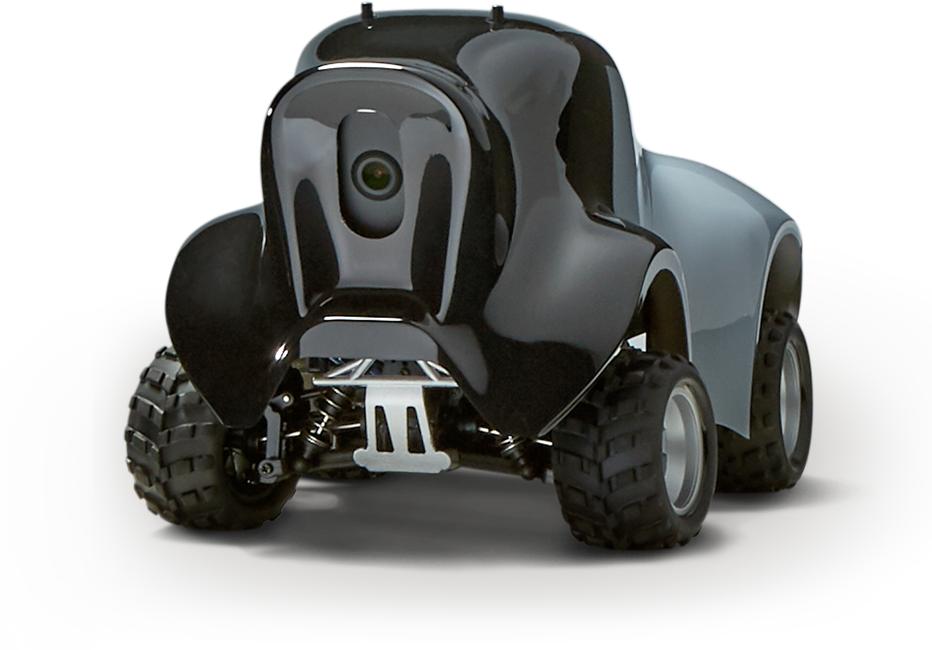
\includegraphics[width=0.5\linewidth]{images/DeepRacer.png}
    \caption{The AWS DeepRacer Car}
    \label{fig:deepcar}
\end{figure}
First announced at the Amazon Web Services (AWS) re:Invent conference in 2018 \citep{Deep18}, the Amazon DeepRacer project \citep{Amz23} provides a way for users to get started with reinforcement learning (RL) - an advanced machine learning technique - by providing a platform which allows a user to implement a self-driving vehicle using RL. The project provides ways for users to learn RL and compare their models with other users. There are three fundamental parts to the project: the Simulator, the Car, and the League.
\\\\
The AWS DeepRacer car \ref{fig:deepcar} is the pinnacle of the DeepRacer project. An autonomous 1/18th scale race car designed to bring an RL model created on the simulator into real-life on a physical race track. Equipped with multiple cameras, an RL model can be put onto the car to control the throttle and steering to safely navigate it around a track. The car is available to buy from Amazon with the current price of \$399 for the basic model \citep{Car}. This can be upgraded to the 'Evo' model by buying a sensor kit for an additional \$249 (or buying the whole Evo car for \$598). Exact details of the car can be found in FIG. The DeepRacer car However, this car is not currently available to buy in the UK.
\\\\
Before an RL model can be used on a DeepRacer car, it needs to be created, trained, and evaluated. This can be done using DeepRacers simulator console. AWS requires that users pay for the training and evaluation time, and the storage for the models. Although the free AWS tier does give enough time to users to train and evaluate their first model, for it to hold up to competition standard, they would need to pay for additional training and evaluation time - costing \$3.50 per hour \citep{Price}.
\\\\
These models can eventually be put to the test in AWS's DeepRacer League, where competitors test their models both physically and virtually over the course of a few months to see who’s is best. Branded as the \textit{"world's first global autonomous racing league, open to anyone"} \citep{League}, the competition encourages developers from all around the world to enter. There are multiple rounds to each competition, each having different rules and challenges:
\begin{itemize}
    \item The ranking metric across all rounds is some variation of the total time taken for the vehicle to navigate around the track.
    \item There is usually a mixture of rounds hosted virtually (using a simulator) and rounds hosted physically. This is to allow ease of access into the competition.
    \item Some rounds allow the best lap time to be taken out of multiple attempts, whilst others only allow one attempt.
    \item Their is no strict penalty for navigating off of the track, instead the robot is simply re-placed from just before it navigated off.
    \item Some tracks involve additional challenges such as object avoidance.
\end{itemize}
AWS heavily publicises and promotes these events to encourage as much participation from the community as possible. Hosting some competitions virtually allow developers from around the world to enter, as well as allowing people to host their own events for their local community. They have a blog which details information about current competitions to keep people up-to-date [CITE]. They also have DeepRacer LIVE [CITE], which is their own system for broadcasting live races. Additionally, they also host competitions for students which gives a more affordable option. Finally, they showcase community projects on the DeepRacer website to show the self-driving possibilities. Such examples are the 'Follow the Leader' project [CITE], which allows the DeepRacer car to identify and follow an object, and also the 'Off Road' project [CITE] which allows the car to follow a waypoint marked by a series of QR codes. However, it's main drawback is the eventual pricing.

\subsection{Formula Pi}

\section{Foundational Technologies}
Research into technologies:
UART package
Callums espruino tools?
Pololo Robot
Track Research


%==================================================================================================================================
\chapter{Competition: Analysis/Requirements}
As mentioned in section 1.2, the first stage of the project was to create a low-cost competition for a self-driving robot which anyone could enter from all around the world.
For this to be realised, three fundamental components needed to be produced:
\begin{itemize}
    \item A detailed analysis and descriptions of the competition's structure and rules.
    \item A race-track which competitors submissions will be tested on.
    \item A website, which details the first two points and allows people to enter the competition.
\end{itemize}
This chapter will detail the analysis conducted to develop the competition. It will give a detailed overview of the different functional and non-functional requirements of the three aforementioned components, and how they realise the previously mentioned project aims.

\section{Competition Structure and Rules}
\subsection{Functional Requirements}
To create the self-driving robot competition, multiple functional requirements were identified. It was important that these requirements were clearly defined as they would be integral in helping establish a well-organised and appealing competition. These requirements have no order of precedence and all carry the same level of importance and priority regarding their need towards creating the competition.
\begin{enumerate}[label=A\arabic*]
    \item Scoring system: a clearly defined scoring system should be developed which details exactly how points are allocated to submissions. This should include the criteria upon which points should be awarded, how points should be collated across the competition, and grounds for which points can be deducted.
    \item Schedule: a date and time for the competition should be made so that entrants know when they need to submit their entry.
    \item Submission: there should be clearly defined instructions on how participants can enter the competition.
    \item Stages: the number of stages for the competition should be decided upon early and detail should be given as to how each stage would differ.
    \item Location: it should be clear to participants where the competition is taking place.
    \item Clearly defined rules: a rulebook should be made which extensively describes specific details of the competition. Much of this is encompassed by the points above.
\end{enumerate}

\subsection{Non-Functional Requirements}
Additionally, non-functional requirements were also identified for the competition. Although many of these requirements are not required to make a functioning competition, they are needed to fulfil the aims laid out in section 1.2.
\begin{enumerate}[label=A.\arabic*]
\setcounter{enumi}{6} % Set the counter to start from the next number after the last item in the previous section
    \item Affordable: money should not be a factor when considering entering the competition. The competition should be free to all.
    \item Accessible: the competition should support a wide variety of participants from all over the world.
    \item Collaborative: different ways of allowing people to work together should be advertised.
    \item Scalable: the competition should be able to grow over time, expanding to accommodate more participants.
    \item Interoperability: participants should be able to participate with whatever robot they have available - as long as it adheres to the requirements.
\end{enumerate}

\section{The Track}
Following from the analysis of the overarching competition structure and rules, was the gathering of requirements for the race-track(s). As this is only a small part of the competition, no comprehensive list of requirements was made, instead just a few important key aspects were considered.
\begin{enumerate}[label=\arabic{chapter}.\arabic*]
\setcounter{enumi}{11}
    \item Versatile: whatever the number of tracks, they must be able to adequately test the various methods of controlling the robot. Aligning with the aims in 1.2, there should be no strict requirement for which methods of autonomous driving are used, and so the track(s) should be suitable for different methods.
    \item The environment: when designing the track(s), the environment in which it will be placed should be considered, such as whether it is indoors or outdoors, and the surface it will be placed on.
    \item Easy to construct: the track(s) must be easy to construct so that participants can build it themselves in their own homes.
\end{enumerate}

\section{The Website}
Similar to the competition and rules, requirements were split into functional and non-functional. These requirements were also labelled using the \textit{MoSCoW} acronym. This method labels requirements based off their priority using of the following:
\begin{itemize}
    \item Must Have: requirements which are absolutely critical for creating a minimum viable solution.
    \item Should Have: requirements which are important but not critically essential. 
    \item Could Have: requirements which are desirable but would be acceptable if not implemented.
    \item Won't Have This Time: requirements which could be implemented in the future, however are out of scope of the current project.
\end{itemize}
It should be noted in the following that there is only one level of user considered for the competition. There is no difference in functionality for new/previous participants or for admins of the website.

\subsection{Functional Requirements}
\textit{Must Have}:
\begin{enumerate}[label=\arabic{chapter}.\arabic*]
\setcounter{enumi}{14}
    \item Registration: users must have the ability to register for the competition.
    \item Submission: users must be able to submit their code for their implementation.
    \item Details rules: users must be able to see the rules of the competition.
    \item Competition description: users must be able to view details as to what the competition is.
\end{enumerate}

\textit{Should Have}:
\begin{enumerate}[label=\arabic{chapter}.\arabic*]
\setcounter{enumi}{18}
    \item Tracks: users should be able to see details on the track(s) used for the competition.
    \item Build the tracks: user should be able to view instructions on how to construct the track themselves.
    \item Leaderboards: users should be able to see the leaderboards for the current competition.
\end{enumerate}

\textit{Could Have}:
\begin{enumerate}[label=\arabic{chapter}.\arabic*]
\setcounter{enumi}{21}
    \item Contact: users could be able to find information to contact.
    \item Past competition: users could be able to see the previous competitions that have taken place. This would initially be a placeholder page.
    \item Related projects: users could be able to view and submit their own projects relating to autonomous driving.
\end{enumerate}

\textit{Won't Have This Time}:
\begin{enumerate}[label=\arabic{chapter}.\arabic*]
\setcounter{enumi}{24}
    \item User page: it was decided the website does not yet require a user page to view statistics on a user who has entered the competition.
\end{enumerate}

\subsection{Non-Functional Requirements}
\textit{Must Have}:
\begin{enumerate}[label=\arabic{chapter}.\arabic*]
\setcounter{enumi}{25}
    \item Usable: the website must be easily usable - being easy to use and navigate by users of all levels of proficiency.
    \item Aesthetics: the website should be visually appealing, with an attractive design and layout.
    \item Data compliance: the website should comply with data laws and regulations when gathering data from submissions.
\end{enumerate}

\textit{Should Have}:
\begin{enumerate}[label=\arabic{chapter}.\arabic*]
\setcounter{enumi}{28}
    \item Cross-compatible: the website should be available on a variety of devices, such as desktop and mobile.
\end{enumerate}

\textit{Could Have}:
\begin{enumerate}[label=\arabic{chapter}.\arabic*]
\setcounter{enumi}{29}
    \item Accessible: the website could provide options for customising different options, such as font-size and colour, to help accessibility.
\end{enumerate}

\textit{Won't Have This Time}:
\begin{enumerate}[label=\arabic{chapter}.\arabic*]
\setcounter{enumi}{30}
    \item Analytics: the website could in the future provide helpful analytics showing statistics regarding, the number of participants, average lap time, where participants are from, and other useful statistics.
\end{enumerate}

%==================================================================================================================================
\chapter{Competition: Design}
 
\section{Competition Structure}
With reference to section 3.1, the following design decisions were made in-order to fulfil the requirements for the competition.

\subsection{Location and Schedule}
As previously decided, the competition was to be taken place remotely - there would be no physical location for participants to travel to. This was done in alignment with the aim of allowing anyone from around the world to easily compete - without forcing any form of physical participation. Additionally, it was decided that there would not yet be any strict start or end date to the competition. Instead, participants could enter when they wished.

\subsection{Stages}
To ensure that participants of all levels of expertise could participate, it was decided to split the competition into multiple stages, with each stage getting incrementally harder and testing a different aspect of a self-driving robot. These stages can be seen in FIG.


\subsection{Competition Entry}
For an entry to be considered, four things are required from a participant:
\begin{enumerate}
    \item Full name: to rank them on the leaderboard.
    \item Contact email: to inform them of any updates.
    \item Country: for potential future analytical purposes.
    \item Link to controller: to test their implementation.
\end{enumerate}
By entering the competition, a participant agrees to make their submission open-source, meaning anyone can view, use, and alter their code to their liking. Therefore, entrants are asked to provide all files relating to their implementation, including instructions on how to use.

\begin{table}[]
\caption{The 10 stages defined for the competition. Each stages has a number, method of control (manual or autonomous), what challenge it will address, and how much of the overall track it will use.}
\label{tab:stages}
\begin{tabular}{@{}|c|c|c|c|c|@{}}
\toprule
\multicolumn{1}{|c|}{\textbf{Stage}} & \multicolumn{1}{c|}{\textbf{Method of Control}} & \multicolumn{1}{c|}{\textbf{Track Section}} & \multicolumn{1}{c|}{\textbf{Challenge}} \\ \midrule
1 & Manual & Straight Line & None \\
2 & Autonomous & Straight Line & None \\
3 & Manual & Full Track & None \\
4 & Autonomous & Full Track & None \\
5 & Manual & Full Track & Obstacles \\
6 & Autonomous & Full Track & Obstacles \\
7 & Manual & Full Track & Parking \\
8 & Autonomous & Full Track & Parking \\
9 & Manual & Full Track & Obstacles+Parking \\
10 & Autonomous & Full Track & Obstacles+Parking \\
\bottomrule
\end{tabular}
\end{table}

\subsection{Scoring System}
Aligning with most other robot competitions (as previously mentioned in section …), each submission would be judged by how fast it could navigate the track at each stage. Three attempts will be taken at each stage, then the best time will be recorded as the official time for that contestant. For simplicity, the timings would be recorded with only a stopwatch. Each stage would have a leaderboard and a competitor's rank on the leaderboard would allocate them a score which is collated for the overall competition.
\\\\
To dissuade any cheating, it was decided that if part of the robot passed over the track edges at any point, a time penalty of +2 seconds would be added to the overall time for that stage. Additionally, if the robot were to fully cross the edge line, then it would be disqualified from that stage, but would still be allowed to compete in later stages. The term “part-of” is difficult to define as there is no simple way to detect how much of a robot has gone over an edge. Therefore, it was concluded that a “judge” would watch the robot navigate the track and would decide on a case-by-case basis upon penalties and disqualifications.
\\\\
To ensure fairness and consistency, all implementations would be tested and timed personally. This avoided the issue of contestants having to time their own submission and had the unofficial additional benefit of testing the ability for the controller to be used by a new user. Additionally, it was deemed that very few people would realistically enter the competition, therefore it was realistic that there would be enough time to individually test every submission.

\section{Track Design}
Following from the requirements listed in 3.2, the following design was created for a race-track. It was decided only a singular track would be used for the competition, instead of multiple tracks for different stages. This was to support the requirement of being easy to construct. The main challenge was designing a track which could accommodate all the various techniques used for autonomous driving (aligning with the requirement regarding versatility). Figure ?? shows the final track design. The intended size of this track would be the size of an A0 sheet of paper (841 x 1189mm). There were multiple reasons for this: firstly it allows the track to be constructed by those who don’t have access to A0 paper by using either 16 sheets of A4 or 8 sheets of A3. Additionally, as the track is intended to be placed indoors, it is large enough to fit the robot on (including any potential obstacles), and small enough to fit inside a standard room.
\\
EXPLAIN PARTS OF TRACK SUCH AS RED BORDERS, MIDDLE LINE, ETC.

\begin{figure}
    \centering
    
\includegraphics[width=0.5\linewidth]{images/final_track_design.png}
    \caption{The Final design of the race-track}
    \label{fig:deepcar}
\end{figure}

\section{Website}
Wireframes made for the website can be found in APPENDIX. These were designed using Figma - a collaborative interface design tool (REFERENCE). These wireframes were aimed to reflect the requirements previously gathered for the website and to inform the implementation process.

%==================================================================================================================================
\chapter{Competition: Implementation}
As the competition stage was intended to be completed by two students, certain decisions were made to accommodate the skills of both students, regarding the scope and technologies used to design and implement the website. These are outlined in the following section; however, it should be noted that the final website was fully designed and implemented individually.

\section{Languages}
Following from the requirements elicitation, the website was scoped to be implemented statically, using a combination of simple HTML, CSS, and JavaScript. Originally ReactJS - a front-end JavaScript library - was considered for building the website. This was because it allows for easy creation of common UI components. However, the other student working on the project did not feel comfortable using a language that they themselves were not proficient in. Additionally, due to time restrictions for the project, only a couple of weeks were allocated to implementing the website. This meant there would not be enough time to learn any new programming languages out of our expertise, or to implement any of the dynamic features previously scoped.

\section{Hosting}
From these decisions, Github pages was chosen as an appropriate hosting platform. This was due to multiple benefits which it provides:
\begin{itemize}
    \item It allows for free hosting of static websites, meaning no money would have to be spent.
    \item It integrates with Git version control, meaning it’s easy to collaborate with and track changes.
    \item It greatly simplifies the deployment process as all the necessary code is already kept on the Github platform.
\end{itemize}

\section{Final Implementation}
Due to the simplicity of the website, the final implementation was mostly trivial. However, there are a few notable components.

\subsection{Tracks}
A sliding carousel was implemented to show each track
\\\\
STILL TO COMPLETE


%==================================================================================================================================
\chapter{Controller: Analysis/Requirements}
The second stage of the project was to independently develop a controller for the robot to be entered as a submission into the competition. The two main purposes of this controller is to allow the robot to be manually controlled, and to enable self-driving features which would allow the robot to drive autonomously around the track. To understand how to approach this problem, we consider an individual who wishes to enter the competition and needs to develop and test their implementation on the device they have available to them. We aim to understand how this individual fulfils the requirements laid out by the competition, such as constricting the controller to run on a web-page, and also make their controller compatible not only with their own robot, but with the robot used in the competition. This chapter will give a detailed overview of the analysis conducted to elicit the requirements of such a controller. 

\section{Working with the Robot}
STILL TO DO

\section{Working with a Smartphone}
STILL TO DO

\section{Requirements of the Controller}
Multiple requirements were identified for the robot controller. The following section divides these requirements into three sections - requirements for the entire controller, then requirements specific to the manual and autonomous controller components.

\subsection{Controller as a Whole}
Similar to section 3, the requirements gathered in this section can be split into functional and non-functional. Again, the MoSCoW acronym is used, however, most requirements have a \textit{‘Must Have’} priority. Therefore, the requirements that have not been deemed to be absolutely necessary, have been labelled as \textit{‘Could Have’}.

\subsubsection{Functional Requirements}
\textit{Must Have}:
\begin{enumerate}[label=\arabic{chapter}.\arabic*]
    \item Connect to robot: the user must be able to connect to a robot via bluetooth.
    \item Switch-driving mode: the user must be able to switch between manual driving mode and autonomous driving mode.
    \item Start/Stop: the user must be able to start and stop the movement of the robot at any time.
    \item Web-page: the user must be able to use the controller to its full functionality from a web-page.
    \item Inter-operable: the user must be able to use the controller with any device within the constraints previously mentioned in section ??.
\end{enumerate}

\textit{Could Have}:
\begin{enumerate}[label=\arabic{chapter}.\arabic*]
    \item Check battery: the user could be able to check the current battery percentage of the connected robot.
    \item Customise settings: the user could be able to customise various settings of the control to aid accessibility.
\end{enumerate}

\subsubsection{Non-Functional Requirements}
\begin{enumerate}[label=\arabic{chapter}.\arabic*]
    \item Responsive: the controller must be responsive - giving quick, real-time feedback to the user, and responding instantly to the users actions.
    \item Low latency: the controller must be able to send instructions to the robot to be processed almost instantaneously.
    \item Effective UI: the controller must be easy to learn and use, with an aesthetically appealing design.
\end{enumerate}

\subsection{Manual Controller}
The following requirements are those specific to the manual controller. Only functional requirements have been gathered here as this component shares all non-functional requirements required from the controller as a whole.
\begin{enumerate}[label=\arabic{chapter}.\arabic*]
    \item Control manually: the user must be able to use a manual control method to control the robot’s movement.
    \item Control speed: the user must be able to accurately control the robot’s speed using the manual control.
    \item Control steering: the user must be able to accurately control the robot’s steering using the manual control.
\end{enumerate}

\subsection{Autonomous Controller}
Similar to the manual controller requirements, only additional functional requirements specific for the autonomous controller are listed. In this section, the controller can be considered to be the user ‘driving’ the robot. Therefore, the term  \textit{‘user’} specifically refers to manual inputs from the individual using the program, while the term \textit{‘controller’} refers to automated decisions made by the program.
\begin{enumerate}[label=\arabic{chapter}.\arabic*]
    \item Control autonomously: the user must be able to use the autonomous driving mode to let the robot drive itself around the track.
    \item Self-driving method: the user must be able to select a combination of autonomous driving methods to allow the robot to drive autonomously. Examples of such methods are colour detection, and line-detection.
    \item Object detection: the controller must be able to detect objects on the race-track.
    \item Object avoidance: the controller must be able to safely navigate the robot around detected objects, whilst staying within the confines of the track.
    \item Connect to camera: the user must be able to connect to a camera on a device.
    \item Process inputs: the controller must be able to process the inputs given by a camera and relate such inputs to its given self-driving method.
\end{enumerate}

%==================================================================================================================================
\chapter{Guidance}
What did you do to implement this idea, and what technical achievements did you make?
\section{Guidance}
You can't talk about everything. Cover the high level first, then cover important, relevant or impressive details.



\section{General points}

These points apply to the whole dissertation, not just this chapter.



\subsection{Figures}
\emph{Always} refer to figures included, like Figure \ref{fig:relu}, in the body of the text. Include full, explanatory captions and make sure the figures look good on the page.
You may include multiple figures in one float, as in Figure \ref{fig:synthetic}, using \texttt{subcaption}, which is enabled in the template.



% Figures are important. Use them well.
\begin{figure}
    \centering
    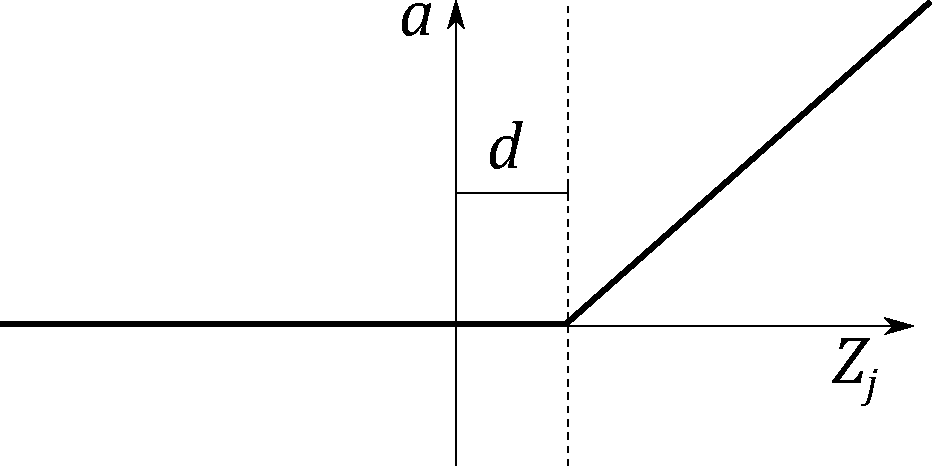
\includegraphics[width=0.5\linewidth]{images/relu.pdf}    

    \caption{In figure captions, explain what the reader is looking at: ``A schematic of the rectifying linear unit, where $a$ is the output amplitude,
    $d$ is a configurable dead-zone, and $Z_j$ is the input signal'', as well as why the reader is looking at this: 
    ``It is notable that there is no activation \emph{at all} below 0, which explains our initial results.'' 
    \textbf{Use vector image formats (.pdf) where possible}. Size figures appropriately, and do not make them over-large or too small to read.
    }

    % use the notation fig:name to cross reference a figure
    \label{fig:relu} 
\end{figure}


\begin{figure}
    \centering
    \begin{subfigure}[b]{0.45\textwidth}
        
\includegraphics[width=\textwidth]{images/synthetic.png}
        \caption{Synthetic image, black on white.}
        \label{fig:syn1}
    \end{subfigure}
    ~ %add desired spacing between images, e. g. ~, \quad, \qquad, \hfill etc. 
      %(or a blank line to force the subfigure onto a new line)
    \begin{subfigure}[b]{0.45\textwidth}
        
\includegraphics[width=\textwidth]{images/synthetic_2.png}
        \caption{Synthetic image, white on black.}
        \label{fig:syn2}
    \end{subfigure}
    ~ %add desired spacing between images, e. g. ~, \quad, \qquad, \hfill etc. 
    %(or a blank line to force the subfigure onto a new line)    
    \caption{Synthetic test images for edge detection algorithms. \subref{fig:syn1} shows various gray levels that require an adaptive algorithm. \subref{fig:syn2}
    shows more challenging edge detection tests that have crossing lines. Fusing these into full segments typically requires algorithms like the Hough transform.
    This is an example of using subfigures, with \texttt{subref}s in the caption.
    }\label{fig:synthetic}
\end{figure}

\clearpage

\subsection{Equations}

Equations should be typeset correctly and precisely. Make sure you get parenthesis sizing correct, and punctuate equations correctly 
(the comma is important and goes \textit{inside} the equation block). Explain any symbols used clearly if not defined earlier. 

For example, we might define:
\begin{equation}
    \hat{f}(\xi) = \frac{1}{2}\left[ \int_{-\infty}^{\infty} f(x) e^{2\pi i x \xi} \right],
\end{equation}    
where $\hat{f}(\xi)$ is the Fourier transform of the time domain signal $f(x)$.

\subsection{Algorithms}
Algorithms can be set using \texttt{algorithm2e}, as in Algorithm \ref{alg:metropolis}.

% NOTE: line ends are denoted by \; in algorithm2e
\begin{algorithm}
    \DontPrintSemicolon
    \KwData{$f_X(x)$, a probability density function returing the density at $x$.\; $\sigma$ a standard deviation specifying the spread of the proposal distribution.\;
    $x_0$, an initial starting condition.}
    \KwResult{$s=[x_1, x_2, \dots, x_n]$, $n$ samples approximately drawn from a distribution with PDF $f_X(x)$.}
    \Begin{
        $s \longleftarrow []$\;
        $p \longleftarrow f_X(x)$\;
        $i \longleftarrow 0$\;
        \While{$i < n$}
        {
            $x^\prime \longleftarrow \mathcal{N}(x, \sigma^2)$\;
            $p^\prime \longleftarrow f_X(x^\prime)$\;
            $a \longleftarrow \frac{p^\prime}{p}$\;
            $r \longleftarrow U(0,1)$\;
            \If{$r<a$}
            {
                $x \longleftarrow x^\prime$\;
                $p \longleftarrow f_X(x)$\;
                $i \longleftarrow i+1$\;
                append $x$ to $s$\;
            }
        }
    }
    
\caption{The Metropolis-Hastings MCMC algorithm for drawing samples from arbitrary probability distributions, 
specialised for normal proposal distributions $q(x^\prime|x) = \mathcal{N}(x, \sigma^2)$. The symmetry of the normal distribution means the acceptance rule takes the simplified form.}\label{alg:metropolis}
\end{algorithm}

\subsection{Tables}

If you need to include tables, like Table \ref{tab:operators}, use a tool like https://www.tablesgenerator.com/ to generate the table as it is
extremely tedious otherwise. 

\begin{table}[]
    \caption{The standard table of operators in Python, along with their functional equivalents from the \texttt{operator} package. Note that table
    captions go above the table, not below. Do not add additional rules/lines to tables. }\label{tab:operators}
    %\tt 
    \rowcolors{2}{}{gray!3}
    \begin{tabular}{@{}lll@{}}
    %\toprule
    \textbf{Operation}    & \textbf{Syntax}                & \textbf{Function}                            \\ %\midrule % optional rule for header
    Addition              & \texttt{a + b}                          & \texttt{add(a, b)}                                    \\
    Concatenation         & \texttt{seq1 + seq2}                    & \texttt{concat(seq1, seq2)}                           \\
    Containment Test      & \texttt{obj in seq}                     & \texttt{contains(seq, obj)}                           \\
    Division              & \texttt{a / b}                          & \texttt{div(a, b) }  \\
    Division              & \texttt{a / b}                          & \texttt{truediv(a, b) } \\
    Division              & \texttt{a // b}                         & \texttt{floordiv(a, b)}                               \\
    Bitwise And           & \texttt{a \& b}                         & \texttt{and\_(a, b)}                                  \\
    Bitwise Exclusive Or  & \texttt{a \textasciicircum b}           & \texttt{xor(a, b)}                                    \\
    Bitwise Inversion     & \texttt{$\sim$a}                        & \texttt{invert(a)}                                    \\
    Bitwise Or            & \texttt{a | b}                          & \texttt{or\_(a, b)}                                   \\
    Exponentiation        & \texttt{a ** b}                         & \texttt{pow(a, b)}                                    \\
    Identity              & \texttt{a is b}                         & \texttt{is\_(a, b)}                                   \\
    Identity              & \texttt{a is not b}                     & \texttt{is\_not(a, b)}                                \\
    Indexed Assignment    & \texttt{obj{[}k{]} = v}                 & \texttt{setitem(obj, k, v)}                           \\
    Indexed Deletion      & \texttt{del obj{[}k{]}}                 & \texttt{delitem(obj, k)}                              \\
    Indexing              & \texttt{obj{[}k{]}}                     & \texttt{getitem(obj, k)}                              \\
    Left Shift            & \texttt{a \textless{}\textless b}       & \texttt{lshift(a, b)}                                 \\
    Modulo                & \texttt{a \% b}                         & \texttt{mod(a, b)}                                    \\
    Multiplication        & \texttt{a * b}                          & \texttt{mul(a, b)}                                    \\
    Negation (Arithmetic) & \texttt{- a}                            & \texttt{neg(a)}                                       \\
    Negation (Logical)    & \texttt{not a}                          & \texttt{not\_(a)}                                     \\
    Positive              & \texttt{+ a}                            & \texttt{pos(a)}                                       \\
    Right Shift           & \texttt{a \textgreater{}\textgreater b} & \texttt{rshift(a, b)}                                 \\
    Sequence Repetition   & \texttt{seq * i}                        & \texttt{repeat(seq, i)}                               \\
    Slice Assignment      & \texttt{seq{[}i:j{]} = values}          & \texttt{setitem(seq, slice(i, j), values)}            \\
    Slice Deletion        & \texttt{del seq{[}i:j{]}}               & \texttt{delitem(seq, slice(i, j))}                    \\
    Slicing               & \texttt{seq{[}i:j{]}}                   & \texttt{getitem(seq, slice(i, j))}                    \\
    String Formatting     & \texttt{s \% obj}                       & \texttt{mod(s, obj)}                                  \\
    Subtraction           & \texttt{a - b}                          & \texttt{sub(a, b)}                                    \\
    Truth Test            & \texttt{obj}                            & \texttt{truth(obj)}                                   \\
    Ordering              & \texttt{a \textless b}                  & \texttt{lt(a, b)}                                     \\
    Ordering              & \texttt{a \textless{}= b}               & \texttt{le(a, b)}                                     \\
    % \bottomrule
    \end{tabular}
    \end{table}
\subsection{Code}

Avoid putting large blocks of code in the report (more than a page in one block, for example). Use syntax highlighting if possible, as in Listing \ref{lst:callahan}.

\begin{lstlisting}[language=python, float, caption={The algorithm for packing the $3\times 3$ outer-totalistic binary CA successor rule into a 
    $16\times 16\times 16\times 16$ 4 bit lookup table, running an equivalent, notionally 16-state $2\times 2$ CA.}, label=lst:callahan]
    def create_callahan_table(rule="b3s23"):
        """Generate the lookup table for the cells."""        
        s_table = np.zeros((16, 16, 16, 16), dtype=np.uint8)
        birth, survive = parse_rule(rule)

        # generate all 16 bit strings
        for iv in range(65536):
            bv = [(iv >> z) & 1 for z in range(16)]
            a, b, c, d, e, f, g, h, i, j, k, l, m, n, o, p = bv

            # compute next state of the inner 2x2
            nw = apply_rule(f, a, b, c, e, g, i, j, k)
            ne = apply_rule(g, b, c, d, f, h, j, k, l)
            sw = apply_rule(j, e, f, g, i, k, m, n, o)
            se = apply_rule(k, f, g, h, j, l, n, o, p)

            # compute the index of this 4x4
            nw_code = a | (b << 1) | (e << 2) | (f << 3)
            ne_code = c | (d << 1) | (g << 2) | (h << 3)
            sw_code = i | (j << 1) | (m << 2) | (n << 3)
            se_code = k | (l << 1) | (o << 2) | (p << 3)

            # compute the state for the 2x2
            next_code = nw | (ne << 1) | (sw << 2) | (se << 3)

            # get the 4x4 index, and write into the table
            s_table[nw_code, ne_code, sw_code, se_code] = next_code

        return s_table

\end{lstlisting}

%==================================================================================================================================
\chapter{Evaluation} 
How good is your solution? How well did you solve the general problem, and what evidence do you have to support that?

\section{Guidance}
\begin{itemize}
    \item
        Ask specific questions that address the general problem.
    \item
        Answer them with precise evidence (graphs, numbers, statistical
        analysis, qualitative analysis).
    \item
        Be fair and be scientific.
    \item
        The key thing is to show that you know how to evaluate your work, not
        that your work is the most amazing product ever.
\end{itemize}

\section{Evidence}
Make sure you present your evidence well. Use appropriate visualisations, reporting techniques and statistical analysis, as appropriate.

If you visualise, follow the basic rules, as illustrated in Figure \ref{fig:boxplot}:
\begin{itemize}
\item Label everything correctly (axis, title, units).
\item Caption thoroughly.
\item Reference in text.
\item \textbf{Include appropriate display of uncertainty (e.g. error bars, Box plot)}
\item Minimize clutter.
\end{itemize}

See the file \texttt{guide\_to\_visualising.pdf} for further information and guidance.

\begin{figure}
    \centering
    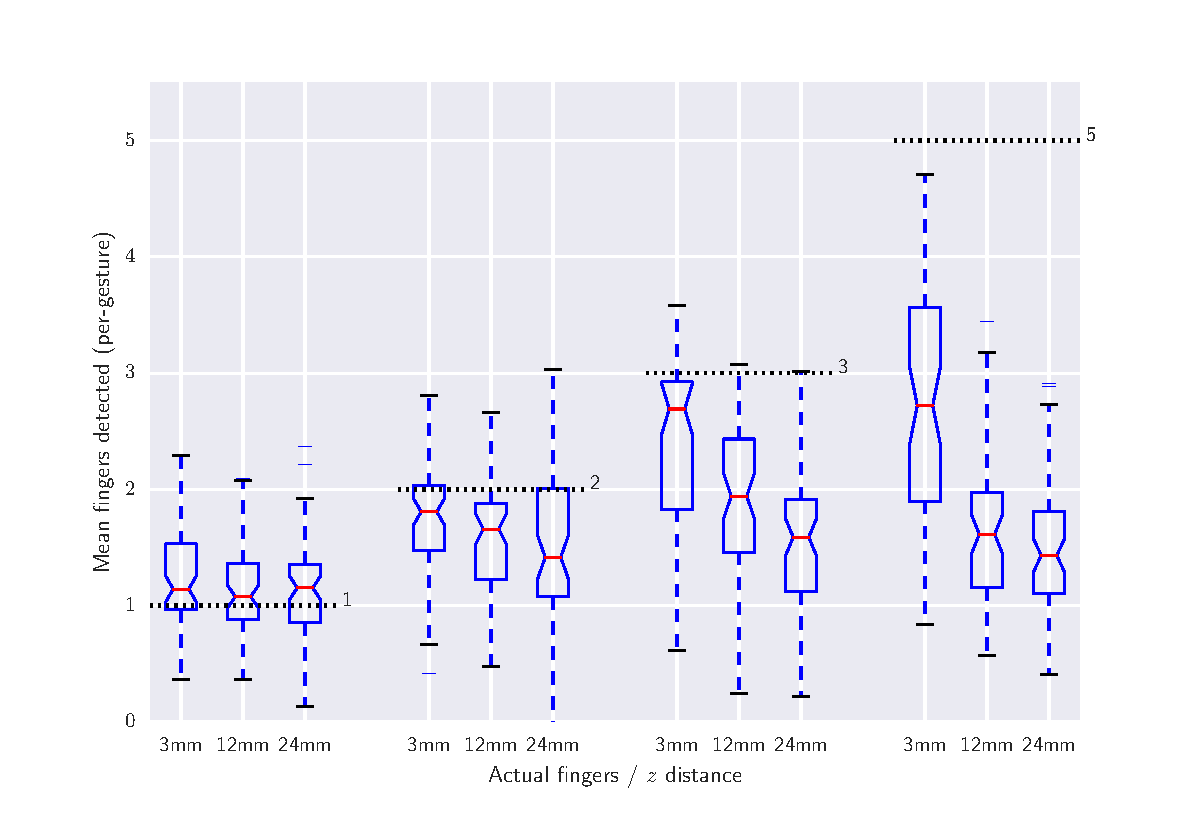
\includegraphics[width=1.0\linewidth]{images/boxplot_finger_distance.pdf}    

    \caption{Average number of fingers detected by the touch sensor at different heights above the surface, averaged over all gestures. Dashed lines indicate
    the true number of fingers present. The Box plots include bootstrapped uncertainty notches for the median. It is clear that the device is biased toward 
    undercounting fingers, particularly at higher $z$ distances.
    }

    % use the notation fig:name to cross reference a figure
    \label{fig:boxplot} 
\end{figure}


%==================================================================================================================================
\chapter{Conclusion}    
Summarise the whole project for a lazy reader who didn't read the rest (e.g. a prize-awarding committee).
\section{Guidance}
\begin{itemize}
    \item
        Summarise briefly and fairly.
    \item
        You should be addressing the general problem you introduced in the
        Introduction.        
    \item
        Include summary of concrete results (``the new compiler ran 2x
        faster'')
    \item
        Indicate what future work could be done, but remember: \textbf{you
        won't get credit for things you haven't done}.
\end{itemize}

%==================================================================================================================================
%
% 
%==================================================================================================================================
%  APPENDICES  

\begin{appendices}

\chapter{Appendices}

Typical inclusions in the appendices are:

\begin{itemize}
\item
  Copies of ethics approvals (required if obtained)
\item
  Copies of questionnaires etc. used to gather data from subjects.
\item
  Extensive tables or figures that are too bulky to fit in the main body of
  the report, particularly ones that are repetitive and summarised in the body.

\item Outline of the source code (e.g. directory structure), or other architecture documentation like class diagrams.

\item User manuals, and any guides to starting/running the software.

\end{itemize}

\textbf{Don't include your source code in the appendices}. It will be
submitted separately.

\end{appendices}

%==================================================================================================================================
%   BIBLIOGRAPHY   

% The bibliography style is abbrvnat
% The bibliography always appears last, after the appendices.

\bibliographystyle{abbrvnat}

\bibliography{l4proj}

\end{document}
